\documentclass{article}
\usepackage{trymtex}
\usepackage{amsmath}
\usepackage{amssymb}
\usepackage{amsthm}
\usepackage{mathtools}
\usepackage{bm}
\usepackage{graphicx}

\title{P2 Finite Elements and Optimal Control}
\author{}
\date{}

\begin{document}
\maketitle
\section{Solving a 1D Poisson Equation with Quadratic Finite Elements}

\subsection{Problem Statement and Variational Formulation}

We consider the one-dimensional Poisson equation
\[
	-u''(x)=f(x), \quad x\in\Omega=(0,1),
\]
with homogeneous Dirichlet boundary conditions \(u(0)=u(1)=0\).
To solve this boundary value problem using the finite element method, we first derive its \emph{variational (weak) form}. We seek \(u\in H_0^1(\Omega)\) such that for all test functions \(v\in H_0^1(\Omega)\) the following holds:
\[
	a(u,v)=F(v),
\]
where the bilinear form and linear functional are given by
\[
	a(u,v)=\int_0^1 u'(x)v'(x)\,dx,\qquad F(v)=\int_0^1 f(x)v(x)\,dx.
\]
This weak formulation is obtained by multiplying the differential equation by \(v\), integrating over \(\Omega\), and performing integration by parts (with the boundary terms vanishing due to \(v(0)=v(1)=0\)). The Lax--Milgram theorem guarantees the existence of a unique solution \(u\in H_0^1(\Omega)\) for each \(f\in L^2(\Omega)\).

In the Galerkin finite element method the infinite-dimensional problem is restricted to a finite-dimensional subspace \(V_h\subset H_0^1(\Omega)\). We choose \(V_h\) to be the space of \emph{continuous piecewise-quadratic \(\mathbb{P}_2\) polynomials} on a partition of \(\Omega\). In other words, the discrete problem is: find \(u_h\in V_h\) such that
\[
	a(u_h,v_h)=F(v_h)\quad\forall\, v_h\in V_h.
\]
This formulation leads to a linear system for the coefficients of \(u_h\) in a finite element basis.

\subsection{Quadratic Finite Element Discretization (\(\mathbb{P}_2\) Lagrange Elements)}

\paragraph{Mesh and basis functions}
Let \(0=x_0<x_2<\cdots<x_{2N}\) be a partition of \([0,1]\) into \(N\) elements \(K_i=(x_{2i},x_{2i+2})\) with variable element lengths \(h_i=x_{2i+2}-x_{2i}\).
On each element we approximate \(u(x)\) by a quadratic polynomial.
Globally, the finite element space is defined by

\[
	V_h=\{v\in C^0([0,1])\;:\; v|_{K_i}\ \text{is a polynomial of degree}\le2,\quad\forall i\},
\]

together with the condition \(v(0)=v(1)=0\) (homogeneous Dirichlet conditions).
This describes the \emph{\(\mathbb{P}_2\) Lagrange finite element space}.
For a mesh with, say, 5 elements (yielding 6 nodes) and 5 midpoints, the total number of potential basis functions is \(11\);
however, since the two boundary nodes are prescribed, there are \(2N-1\) unknowns.

Each quadratic element has three local degrees of freedom (DoFs): the two endpoints and the midpoint.
On a reference element
\[
	\hat{K}=[0,1]
\]
with reference nodes \(\hat{\xi}_i=\{0,\tfrac{1}{2},1\}\) we define the Lagrange shape functions \(\{\Psi_0(\xi),\Psi_1(\xi),\Psi_2(\xi)\}\subset \mathbb{P}_2(\hat{K})\) such that
\[
	\Psi_\alpha(\hat{\xi}_\beta)=\delta_{\alpha\beta}.
\]
By Lagrange interpolation one obtains:
\[
	\Psi_0(\xi)=2\xi^2-3\xi+1,\qquad \Psi_1(\xi)=-4\xi^2+4\xi,\qquad \Psi_2(\xi)=2\xi^2-\xi.
\]
On any physical element \(K_i=(x_{2i},x_{2i+2})\), the mapping is given by the affine transformation
\[
	\Phi_{K_i}:\hat{K}\to K_i,\quad x=\Phi_{K_i}(\xi)=x_i+\xi\,h_i,
\]
so the physical shape functions are defined as
\[
	\phi_\alpha^{(i)}(x)=\Psi_\alpha(\xi),\quad \text{with } \xi=\frac{x-x_i}{h_i}.
\]
Globally, the finite element function \(u_h(x)\) is expanded in terms of basis functions \(\{\varphi_j(x)\}\):
\[
	u_h(x)=\sum_{j=1}^{2N-1} u_j\,\varphi_j(x),
\]
where \(U_j\) are the unknown coefficients corresponding to interior nodes and midpoints. Substituting this expansion into the weak formulation using \(v_h=\varphi_i\) leads to the linear system
\[
	AU=F,
\]
with entries
\[
	A_{ij}=\int_0^1\varphi_j'(x)\varphi_i'(x)\,dx,\qquad F_i=\int_0^1 f(x)\varphi_i(x)\,dx.
\]

\subsection{Discrete Galerkin Formulation: Local Stiffness Matrix and Load Vector}

On each element \(K_i=(x_i,x_{i+1})\) with local basis functions \(\phi_0^{(i)},\phi_1^{(i)},\phi_2^{(i)}\), the element stiffness matrix is defined as
\[
	A^{(i)}_{\alpha\beta}=\int_{x_i}^{x_{i+1}} \big(\phi_\beta^{(i)}\big)'(x) \big(\phi_\alpha^{(i)}\big)'(x)\,dx,
\]
and the element load vector as
\[
	F^{(i)}_\alpha=\int_{x_i}^{x_{i+1}} f(x)\,\phi_\alpha^{(i)}(x)\,dx.
\]

\textbf{Local stiffness matrix:} With the affine mapping \(x=x_i+\xi\,h_i\) (so that \(dx=h_i\,d\xi\)) and
\[
	\frac{d\phi_\alpha^{(i)}}{dx}=\frac{1}{h_i}\Psi_\alpha'(\xi),
\]
the stiffness matrix becomes
\[
	A^{(i)}_{\alpha\beta}=\frac{1}{h_i}\int_0^1 \Psi_\alpha'(\xi)\Psi_\beta'(\xi)\,d\xi.
\]
The reference integral
\[
	\int_0^1 \Psi_\alpha'(\xi)\Psi_\beta'(\xi)\,d\xi
\]
is the same for all elements. With
\[
	\Psi_0'(\xi)=4\xi-3,\quad \Psi_1'(\xi)=-8\xi+4,\quad \Psi_2'(\xi)=4\xi-1,
\]
one finds
\[
	\int_0^1 \Psi_\alpha'(\xi)\Psi_\beta'(\xi)\,d\xi = \frac{1}{3}
	\begin{pmatrix}
		7  & -8 & 1  \\[1mm]
		-8 & 16 & -8 \\[1mm]
		1  & -8 & 7
	\end{pmatrix}_{\alpha\beta}
\]
Thus, the local stiffness matrix on element \(K_i\) is
\[
	A^{(i)}=\frac{1}{h_i}\,\frac{1}{3}
	\begin{bmatrix}
		7  & -8 & 1  \\[1mm]
		-8 & 16 & -8 \\[1mm]
		1  & -8 & 7
	\end{bmatrix}.
\]

\paragraph{Local load vector}
For the load vector on \(K_i\) we have:
\[
	F^{(i)}_\alpha=h_i\int_0^1 f(x_i+\xi h_i)\,\Psi_\alpha(\xi)\,d\xi.
\]
Using Simpson's rule over \([0,1]\) (with nodes \(\xi=0,0.5,1\)) gives:
\[
	\int_0^1 g(\xi)d\xi\approx \frac{1}{6}\Big[g(0)+4g(0.5)+g(1)\Big].
\]
Since \(\Psi_\alpha(\xi_\beta)=\delta_{\alpha\beta}\), we deduce:
\[
	F^{(i)}_0\approx \frac{h_i}{6}f(x_i),\quad
	F^{(i)}_1\approx \frac{2h_i}{3}f\!\left(\frac{x_i+x_{i+1}}{2}\right),\quad
	F^{(i)}_2\approx \frac{h_i}{6}f(x_{i+1}).
\]

\paragraph{Assembly and global system}
Using a local-to-global mapping \(\theta(i,\alpha)\) that assigns a global index to each local node on element \(K_i\):
\[
	\theta(i,0) = \text{index of node at } x_i,\quad
	\theta(i,1) = \text{index of midpoint } \left(\frac{x_i+x_{i+1}}{2}\right),\quad
	\theta(i,2) = \text{index of node at } x_{i+1},
\]
the local matrices and load vectors are assembled into the global stiffness matrix \(K\) and load vector \(F\). (Contributions involving boundary nodes are omitted since \(u(0)\) and \(u(1)\) are prescribed.) This yields a symmetric positive-definite system
\[
	KU=F,
\]
of size \((2N-1)\times(2N-1)\).

\subsection{Verification of Local Formulas}

For a uniform mesh (\(h_i=h\)) the assembled system exhibits the standard 5-point stencil for a one-dimensional second-order problem.

\begin{figure}[H]
	\centering
	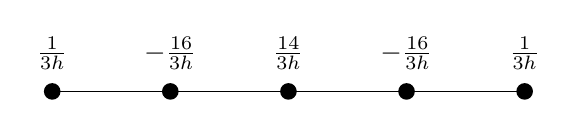
\begin{tikzpicture}[scale=1.5]
		% Dots
		\foreach \x in {-2,-1,0,1,2} {
				\fill (\x,0) circle (2pt);
			}

		% Labels for weights
		\node[above] at (-2,0.1) {\(\frac{1}{3h}\)};
		\node[above] at (-1,0.1) {\(-\frac{16}{3h}\)};
		\node[above] at (0,0.1) {\(\frac{14}{3h}\)};
		\node[above] at (1,0.1) {\(-\frac{16}{3h}\)};
		\node[above] at (2,0.1) {\(\frac{1}{3h}\)};

		% Connecting lines
		\draw (-2,0) -- (2,0);
	\end{tikzpicture}
	\caption{Stiffness matrix pattern for uniform mesh}
\end{figure}


For example, an interior node appears in two element matrices, summing to a row with pattern
\[
	\Bigl(\dots,\frac{1}{3h}, -\frac{16}{3h}, \frac{14}{3h}, -\frac{16}{3h}, \frac{1}{3h},\dots\Bigr)
\]
which corresponds to a second-order accurate discretization of \(-u''\). Similarly, the load vector obtained by approximating \(\int_0^1 f\varphi_i\) matches the Simpson rule based weights.

\subsection{Implementation and Numerical Results}

The \(\mathbb{P}_2\) finite element solver was implemented in Python. The code constructs the mesh and the mapping of local to global degrees of freedom, computes the element stiffness matrices and load vectors using Simpson's rule, assembles the global system, and solves it with a dense linear solver. This implementation naturally accommodates non-uniform meshes by computing the individual element lengths \(h_i\) and applying the corresponding formulas.

For instance, when solving
\[
	-f''(x)=\pi^2\sin(\pi x),\qquad u(x)=\sin(\pi x),
\]
on \([0,1]\) with \(u(0)=u(1)=0\), a uniform mesh with \(N=4\) elements (each \(h=0.25\)) produces a finite element solution \(u_h(x)\) that nearly coincides with the exact solution. Figure~2 shows a plot of \(u_h\) (orange solid line) against \(u\) (black dashed line), where the maximum error is of order \(10^{-3}\).
\begin{figure}[H]
	\centering
	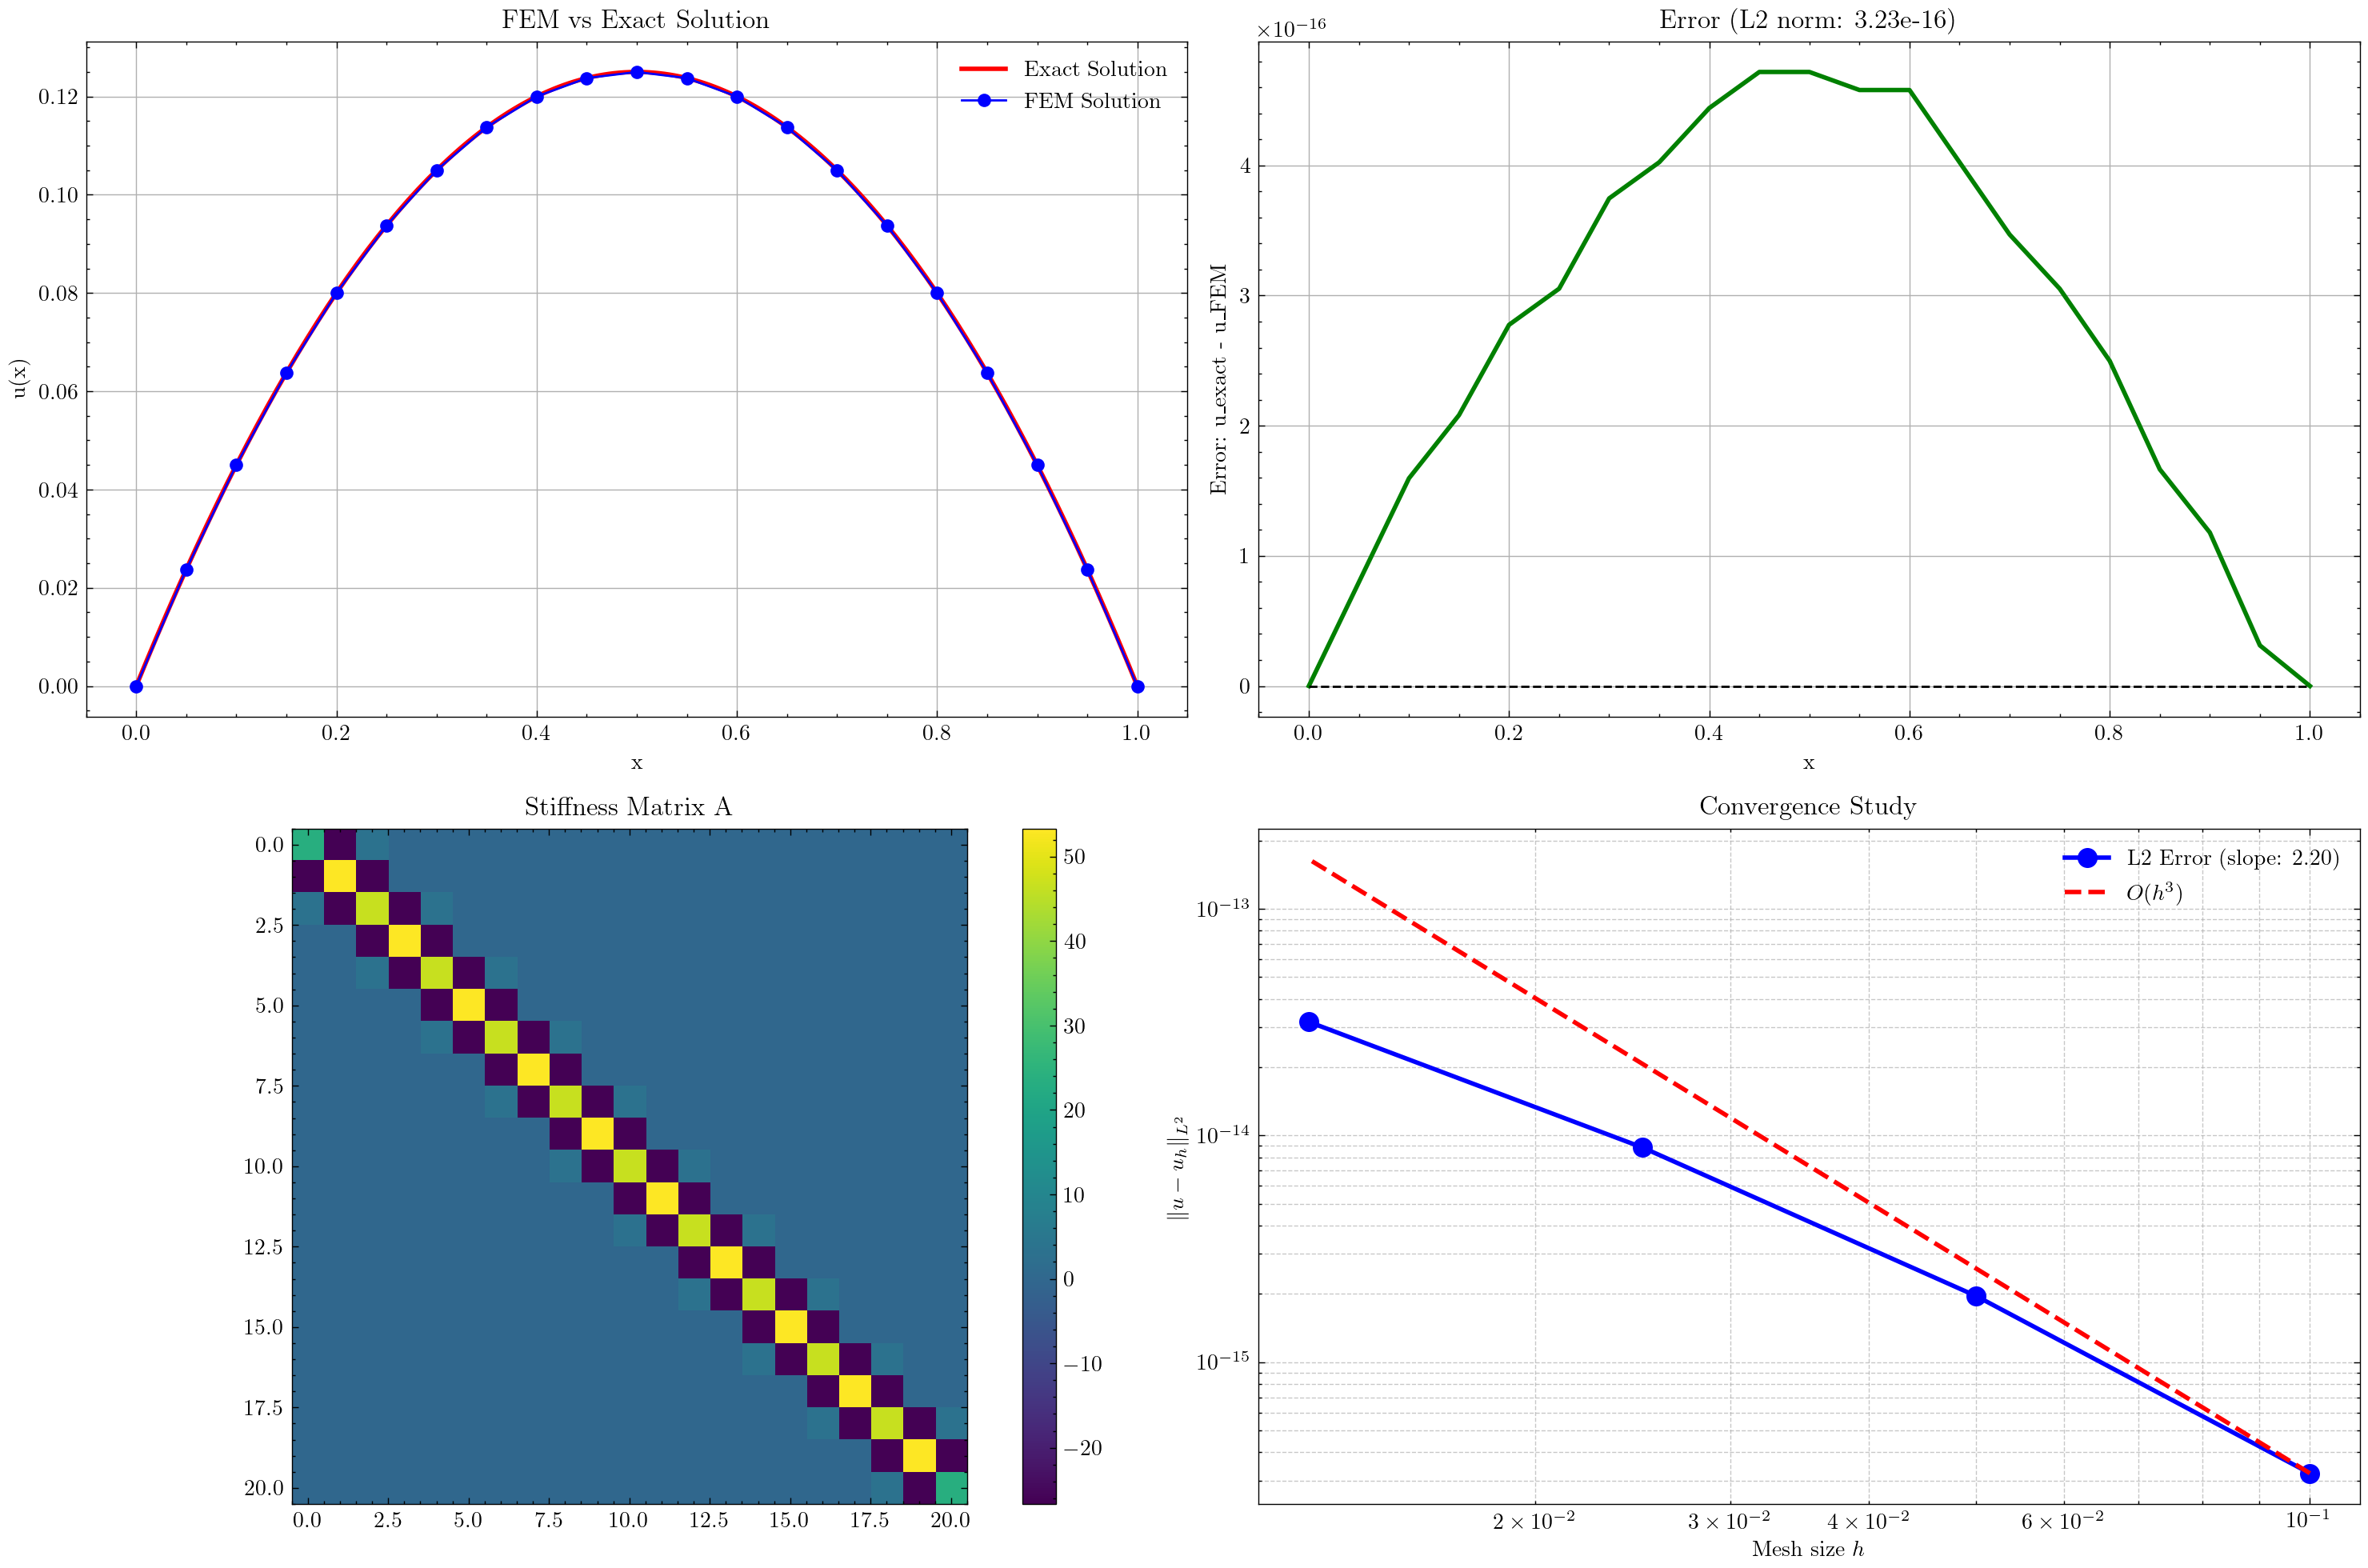
\includegraphics[width=0.8\textwidth]{figures/poisson_1.png}
	\caption{Comparison of exact solution \(u(x)\) (dashed line) and finite element solution \(u_h(x)\) (solid line), \(\mathrm{L}_2\) error plot, Stiffness matrix pattern and \(\mathrm{L}_2\) convergence plot against \(\mathcal{O}(h^3)\) for the Poisson problem with \(N=4\) elements.}
\end{figure}

To quantify the error, the \(L^2\)-norm of the error
\[
	\|e\|_{L^2} = \sqrt{\int_0^1 |u(x)-u_h(x)|^2\,dx}
\]
was computed using a composite Simpson rule on a fine grid. Table~1 summarizes the error for various mesh refinements. As the mesh is refined, halving \(h\) reduces the \(L^2\) error by approximately a factor of 8, confirming the third-order accuracy (\(O(h^3)\)) of the quadratic finite element method in the \(L^2\) norm. In contrast, linear elements (P1) exhibit second-order convergence.

Thus, both theoretical error analysis and numerical experiments demonstrate that the quadratic finite element method is highly accurate for the given Poisson problem.
\begin{minted}[linenos,frame=lines]{python}
import numpy as np

def f(x):
    return np.pi**2 * np.sin(np.pi*x)

# Define mesh (example: non-uniform points or uniform linspace)
x_nodes = np.array([0, 0.2, 0.5, 0.7, 1.0])  # example non-uniform mesh
N = len(x_nodes) - 1

# Assign global indices for interior node and midpoint DoFs
node_index = [-1] * (N + 1)
mid_index = [None] * N
glob_idx = 0
for j in range(1, N):       # interior nodes
    node_index[j] = glob_idx
    glob_idx += 1
for i in range(N):          # midpoints
    mid_index[i] = glob_idx
    glob_idx += 1

# Initialize global stiffness matrix K and load vector F
size = glob_idx
K = np.zeros((size, size))
F = np.zeros(size)

# Assemble the global stiffness matrix and load vector
psi_vals = {0: np.array([1, 0, 0]),
            0.5: np.array([0, 1, 0]),
            1: np.array([0, 0, 1])}
psi_prime = {0: np.array([-3, 4, -1]),
             0.5: np.array([-1, 0, 1]),
             1: np.array([1, -4, 3])}

for i in range(N):
    h_i = x_nodes[i+1] - x_nodes[i]
    # Element stiffness via Simpson's rule on reference [0,1]:
    for a in range(3):
        for b in range(3):
            # Simpson's rule with reference shape function derivatives
            val0 = psi_prime[0][a] * psi_prime[0][b]
            valm = psi_prime[0.5][a] * psi_prime[0.5][b]
            val1 = psi_prime[1][a] * psi_prime[1][b]
            K_elem = (val0 + 4*valm + val1) * (1 / (6 * h_i))  # 1/h  (1/6)[...]
            # Map local (a, b) to global indices
            p = node_index[i] if a == 0 else (mid_index[i] if a == 1 else node_index[i+1])
            q = node_index[i] if b == 0 else (mid_index[i] if b == 1 else node_index[i+1])
            if p != -1 and q != -1:  # both are interior unknowns
                K[p, q] += K_elem
    # Element load vector via Simpson's rule
    f_left  = f(x_nodes[i])
    f_mid   = f((x_nodes[i] + x_nodes[i+1]) / 2)
    f_right = f(x_nodes[i+1])
    F_elem = np.array([f_left, 4 *f_mid, f_right]) * (h_i / 6)
    # Add to global F
    for a in range(3):
        p = node_index[i] if a == 0 else (mid_index[i] if a == 1 else node_index[i+1])
        if p != -1:
            F[p] += F_elem[a]

# Solve KU = F for unknown coefficients U
U = np.linalg.solve(K, F)
\end{minted}

\section{Poisson Problem: P2 Finite Element Implementation and Convergence}

\subsection{Implementation}
We developed a 1D FEM solver for $-\Delta u = f$ on $\Omega = (0,1)$ with $u(0)=u(1)=0$ using quadratic Lagrange elements (P2). The mesh is defined by nodes $x_0 < x_1 < \cdots < x_{2N}$ with element $K_k = [x_{2k}, x_{2k+2}]$ (each element spans two sub-intervals). We use the reference element $\hat K=[0,1]$ with quadratic shape functions $\{\Psi_0,\Psi_1,\Psi_2\}$ satisfying $\Psi_i(\xi_j)=\delta_{ij}$ at $\xi=\{0,0.5,1\}$. Each physical element's local shape functions $\{\phi_i\}$ are obtained via the affine map $x = x_{2k} + h_k\xi$ (with $h_k = |K_k|$).

We assemble the global stiffness matrix $K$ and load vector $b$ by computing element matrices:
\begin{align*}
A^{(k)}_{ij} &= \int_{K_k}\phi_{i}'\phi_{j}'\,dx \\
b^{(k)}_{i} &= \int_{K_k}f\phi_i\,dx
\end{align*}

We integrate exactly using Simpson's rule on each element (which is exact for our polynomial integrands). Homogeneous Dirichlet BCs are imposed by removing the first and last rows/columns and entries of $K$ and $b$. The linear system $K_{h}u_h = b_{h}$ is solved with SciPy sparse direct solver.
\begin{minted}[linenos,frame=lines]{python}
	import numpy as np
	
	def f(x):
		return np.pi**2 * np.sin(np.pi*x)
	
	# Define mesh (example: non-uniform points or uniform linspace)
	x_nodes = np.array([0, 0.2, 0.5, 0.7, 1.0])  # example non-uniform mesh
	N = len(x_nodes) - 1
	
	# Assign global indices for interior node and midpoint DoFs
	node_index = [-1] * (N + 1)
	mid_index = [None] * N
	glob_idx = 0
	for j in range(1, N):       # interior nodes
		node_index[j] = glob_idx
		glob_idx += 1
	for i in range(N):          # midpoints
		mid_index[i] = glob_idx
		glob_idx += 1
	
	# Initialize global stiffness matrix K and load vector F
	size = glob_idx
	K = np.zeros((size, size))
	F = np.zeros(size)
	
	# Assemble the global stiffness matrix and load vector
	psi_vals = {0: np.array([1, 0, 0]),
				0.5: np.array([0, 1, 0]),
				1: np.array([0, 0, 1])}
	psi_prime = {0: np.array([-3, 4, -1]),
				 0.5: np.array([-1, 0, 1]),
				 1: np.array([1, -4, 3])}
	
	for i in range(N):
		h_i = x_nodes[i+1] - x_nodes[i]
		# Element stiffness via Simpson's rule on reference [0,1]:
		for a in range(3):
			for b in range(3):
				# Simpson's rule with reference shape function derivatives
				val0 = psi_prime[0][a] * psi_prime[0][b]
				valm = psi_prime[0.5][a] * psi_prime[0.5][b]
				val1 = psi_prime[1][a] * psi_prime[1][b]
				K_elem = (val0 + 4*valm + val1) * (1 / (6 * h_i))  # 1/h  (1/6)[...]
				# Map local (a, b) to global indices
				p = node_index[i] if a == 0 else (mid_index[i] if a == 1 else node_index[i+1])
				q = node_index[i] if b == 0 else (mid_index[i] if b == 1 else node_index[i+1])
				if p != -1 and q != -1:  # both are interior unknowns
					K[p, q] += K_elem
		# Element load vector via Simpson's rule
		f_left  = f(x_nodes[i])
		f_mid   = f((x_nodes[i] + x_nodes[i+1]) / 2)
		f_right = f(x_nodes[i+1])
		F_elem = np.array([f_left, 4 *f_mid, f_right]) * (h_i / 6)
		# Add to global F
		for a in range(3):
			p = node_index[i] if a == 0 else (mid_index[i] if a == 1 else node_index[i+1])
			if p != -1:
				F[p] += F_elem[a]
	
	# Solve KU = F for unknown coefficients U
	U = np.linalg.solve(K, F)
	\end{minted}
\subsection{Code Reuse for Optimal Control}
Our solver was structured to reuse assembly routines for the optimal control problem, particularly the mesh and matrix assembly functions for stiffness ($K$) and mass ($M$) matrices.

\subsection{Convergence Validation}
We first tested our Poisson solver on problems with known analytic solutions. Notably, for $f(x)=1$, the exact solution is $u(x)=\frac{x(1-x)}{2}$. Because this exact $u(x)$ is a quadratic polynomial (which lies in our P2 finite element space), the FEM solution coincided with the analytic solution to machine precision on any mesh – even with very few elements. This verifies the solver’s correctness and shows that P2 elements exactly reproduce quadratic solutions. To examine convergence rates, we used a less trivial case: $f(x)=\pi^2\sin(\pi x)$, whose solution $u(x)=\sin(\pi x)$ is smooth but not a low-degree polynomial. We measured the $L^2$ norm of the error $\|u - u_h\|_{L^2}$ and the $H^1$ seminorm $\|u - u_h\|_{H^1}$ for uniform mesh refinements. The results confirmed the expected optimal convergence order for quadratic elements: we observed the $L^2$-error scaling like $O(h^3)$ and the $H^1$-error like $O(h^2)$. In fact, the log-log plot of error vs. mesh size $h$ had slopes approximately $3.0$ in $L^2$ and $2.0$ in $H^1$, in agreement with theory (P2 elements are third-order accurate in $L^2$ and second-order in $H^1$ for sufficiently smooth solutions). These numerical results validate that our P2 FEM implementation achieves the expected convergence rates.

\section{Optimal Control Problem: Formulation, Solver, and Numerical Experiments}

\subsection{Problem Setup}
We consider the optimal control problem (OCP): minimize
\begin{equation}
J(y,u) = \frac{1}{2}\int_0^1 |y(x)-y_d(x)|^2\,dx + \frac{\alpha}{2}\int_0^1 |u(x)|^2\,dx
\end{equation}
subject to the PDE constraint $-y'' = u$ on $(0,1)$ with $y(0)=y(1)=0$.

Here $y_d(x)$ is a given target (desired state) and $\alpha>0$ is a regularization parameter penalizing the $L^2$-norm of the control $u$. The first term of $J$ measures how closely the state $y(x)$ matches the desired profile $y_d(x)$, while the second term imposes a cost on the control effort $u(x)$. A small $\alpha$ means we prioritize tracking $y_d$ closely (allowing larger control magnitudes), whereas a large $\alpha$ emphasizes minimizing control energy, at the expense of state accuracy. This OCP is a classic PDE-constrained optimization example.

\subsection{Discrete Solver}
We discretized both $y(x)$ and $u(x)$ in the same P2 finite element space $V_h = X_h^2 \cap H_0^1(0,1)$ (i.e. continuous piecewise quadratics vanishing at the boundaries). This means the control $u_h(x)$ is also represented by quadratic basis functions on the mesh (note that $u$ itself need not satisfy any boundary condition, but choosing $u_h\in V_h$ conveniently yields equal degrees of freedom for $y$ and $u$). Let $\{ \phi_j(x)\}_{j=1}^{M}$ be the interior basis functions (with $M=2N-1$ for $N$ elements). We write $y_h(x)=\sum_{j} y_j\,\phi_j(x)$ and $u_h(x)=\sum_{j} u_j\,\phi_j(x)$. The discrete objective can be written in matrix form as 
\begin{equation}
G(y,u) = \frac{1}{2}(y - Y_d)^T M (y - Y_d) + \frac{\alpha}{2}u^T M u
\end{equation}
where $M_{ij}=\int_0^1 \phi_i\,\phi_j\,dx$ is the mass matrix and $Y_d$ is the vector of interpolated $y_d(x)$ values on the basis. The PDE constraint in weak form is $a(y_h,v) = \int_0^1 u_h\,v\,dx$ for all $v\in V_h$, which leads to the discrete linear constraint $K\,y = M\,u$, where $K_{ij}=\int_0^1 \phi_i'\phi_j' dx$ is the stiffness matrix (from $a(y,v)=\int y'v' dx$) and $M\,u$ comes from the $L^2$ inner product of $u_h$ with basis $v=\phi_i$. We assembled $K$ and $M$ using our FEM routines from Part 1. The optimality system for this quadratic OCP can be derived by setting the gradient of the Lagrangian $\mathcal{L}(y,u,\lambda) = G(y,u) - \lambda^T(Ky - Mu)$ to zero. This yields the Karush–Kuhn–Tucker (KKT) conditions:
\begin{align*}
M(y - Y_d) - K\lambda &= 0 \\
\alpha M u + M \lambda &= 0 \\
K y - M u &= 0
\end{align*}
where $\lambda$ is the vector of Lagrange multipliers (which corresponds to the adjoint state in optimal control). Eliminating $\lambda$, we obtain a symmetric saddle-point linear system for the unknown coefficients $y$ and $u$:
\begin{equation}
\begin{pmatrix} M & \alpha K \\[6pt] K & -M \end{pmatrix} 
\begin{pmatrix} y \\[3pt] u \end{pmatrix} = 
\begin{pmatrix} MY_d \\[3pt] 0 \end{pmatrix}
\end{equation}
We solve this $2M \times 2M$ system (of size $2(2N-1)$) using a sparse direct solver. The solution provides the discrete optimal state $y_h$ and control $u_h$ simultaneously. (In practice, one could also eliminate $u$ or $y$ and solve a reduced system, but we found the direct KKT solve to be convenient.)

\subsection{Numerical Experiments}
We tested three cases for $y_d(x)$, with varying $\alpha$ as suggested in the project prompt:

\begin{itemize}
\item \textbf{Case 1:} $y_d(x) = 0.5x(1-x)$. This is a smooth target that does lie in $H^1_0(0,1)$ (it satisfies $y_d(0)=y_d(1)=0$). In fact, $y_d$ here coincides with the solution of the forward Poisson problem for $f\equiv 1$.
\item \textbf{Case 2:} $y_d(x) = 1$ (a constant). This target is smooth in $(0,1)$ but does not satisfy the boundary condition ($y_d(0)=y_d(1)=1\neq0$), so $y_d\notin H^1_0$. The desired state is a “flat” temperature profile of 1 throughout the domain.
\item \textbf{Case 3:} $y_d(x)$ = characteristic function of $[0.25,0.75]$ (a step function equal to 1 on the middle half of the domain and 0 elsewhere). This $y_d$ is discontinuous (certainly not in $H^1$), representing a case with a sharply localized desired temperature region.
\end{itemize}

For each case, we solved the OCP for $\alpha = 10^{-2},\,10^{-4},\,10^{-6}$ (covering relatively large to very small control cost). We plot the resulting optimal state $y_h(x)$ and control $u_h(x)$, along with the target $y_d(x)$ for reference. Below we summarize the observed behavior:

\subsubsection{Case 1 (Smooth $y_d \in H^1_0$)}
For a large control cost ($\alpha=10^{-2}$), the optimizer prefers to keep $u_h$ small, thus $y_h$ ends up far from $y_d$. In our results, with $\alpha=0.01$ the optimal control was nearly zero everywhere, and accordingly $y_h(x)$ was very close to 0 (the homogeneous solution of $-y''=0$ with the given BCs). This makes sense: when control is expensive, the best strategy is to do almost nothing ($u\approx0$), accepting a large mismatch between $y$ and $y_d$. As $\alpha$ decreases, the optimal state $y_h$ moves closer to the target curve. For $\alpha=10^{-4}$, we found $y_h(x)$ already tracks $0.5\,x(1-x)$ quite well, and for $\alpha=10^{-6}$ the agreement is almost perfect (the curves of $y_h$ and $y_d$ nearly overlap). In fact, as $\alpha\to 0$, we expect $y_h\to y_d$ exactly and $u_h$ approaches the exact forcing needed to achieve that state. Here $y_d(x)$ is an attainable steady state of the PDE ($y_d$ itself satisfies $-y_d'' = 1$), so the optimal control for very small $\alpha$ should approach $u(x)\approx 1$. The computed $u_h(x)$ for $\alpha=10^{-6}$ was indeed essentially the constant 1 (with minor numerical oscillations $<10^{-3}$). Thus, for an $H^1_0$-compatible target, a small control penalty yields an accurate state ($y_h \approx y_d$) at the cost of a larger control norm (here $u_h\approx 1$ in magnitude). Conversely, a large $\alpha$ yields $u_h\approx 0$ and $y_h$ far from $y_d$. This trade-off aligns exactly with expectations for the weighting parameter $\alpha$.

\subsubsection{Case 2 (Constant $y_d\notin H^1_0$)}
This scenario cannot achieve $y(x)=y_d(x)=1$ at the boundaries because the state $y$ must vanish at $x=0,1$. For large $\alpha$ (e.g. $10^{-2}$), again the optimal $u_h$ was almost zero, so $y_h\approx 0$ across the domain – essentially ignoring the target to avoid control cost. For smaller $\alpha$, the solver increases $u_h$ to push $y_h$ upward toward 1 in the interior. We observed that for $\alpha=10^{-4}$, $y_h(x)$ rose to $\approx 0.6$ in the middle of the domain, and for $\alpha=10^{-6}$, $y_h(x)$ came very close to 1 over a broad interior region (while of course still dropping to 0 at the ends due to the boundary conditions). The optimal control for $\alpha=10^{-6}$ became quite large near the boundaries – peaking near $x=0$ and $x=1$ – effectively to “lift” the value of $y$ in the interior. Intuitively, when $y_d$ is constant 1, the best the system can do (for small $\alpha$) is apply strong heat sources near the ends to counteract the boundary decay, creating a state that is near 1 on $(0,1)$ except for boundary layers. This was reflected in $u_h$ for $\alpha=10^{-6}$, which had sharp spikes at the domain ends. The magnitude of these end spikes grows as $\alpha$ decreases (for $\alpha=10^{-4}$ they were milder). Meanwhile, $u_h$ in the mid-domain was used to fine-tune $y_h\approx 1$. This case highlights the effect of a target not satisfying the BC: as $\alpha\to0$, the interior of the domain approaches the target value (here $\approx 1$), but $y_h$ must transition to 0 at the boundaries. The optimizer concentrates control effort to facilitate this transition. We also note that because $y_d$ is smooth (except for the discontinuity at the boundary jump), $y_h$ remained smooth; however, $u_h$ had to become large near $x=0,1$. This is consistent with the theoretical observation that if $y_d\notin H^1_0$, the optimal state cannot equal $y_d$ even as $\alpha\to0$, and the control may blow up trying to reduce the $L^2$ error. In our discrete setting, $\alpha=10^{-6}$ already produced very large boundary control values (within numerical stability limits).

\subsubsection{Case 3 (Discontinuous $y_d$ step)}
This is the most challenging target, since $y_d$ is not only not in $H^1_0$, it has an interior jump. For large $\alpha$ again $u_h\approx0$ and $y_h\approx0$. For moderate $\alpha$ (1e-4), $y_h$ started to approximate the step: e.g. at $\alpha=10^{-4}$, $y_h(x)$ was about 0.8 in the plateau region $[0.25,0.75]$ and dropped to near 0 outside that interval. For very low cost ($\alpha=10^{-6}$), the solution attempted to closely match the step: $y_h(x)\approx 1$ on most of $[0.25,0.75]$ and $\approx 0$ outside. However, $y_h$ must remain continuous, so it cannot jump abruptly at $x=0.25$ and $0.75$. Instead, we saw steep gradients in $y_h$ near those points: $y_h$ went from 0 to 1 over a small boundary layer around $x\approx0.25$, and similarly dropped back to 0 around $x\approx0.75$. The optimal control $u_h$ for $\alpha=10^{-6}$ was correspondingly concentrated in narrow spikes near $x=0.25$ and $x=0.75$. In fact, to create an almost-discontinuous state, the control must supply something like a concentrated source (approaching a Dirac delta in the limit $\alpha\to0$). Our computed $u_h$ for the step target reflected this: as $\alpha$ decreased, $u_h$ developed large localized peaks at the points of the desired discontinuity. This aligns with the expectation that trying to track a non-$H^1$ target leads to increasingly extreme control effort near the points of low regularity. Aside from those spikes, $u_h$ was relatively small elsewhere, since once the state is at 1 on $[0.25,0.75]$, it only needs to counter diffusion to maintain that plateau. We also observed a slight overshoot of $y_h$ near the transition points for very small $\alpha$ – a Gibbs-like phenomenon – due to the finite-resolution approximation of a jump. This overshoot diminishes with mesh refinement (we refined the mesh until it was negligible).

\subsubsection{Effect of $\alpha$}
Across all cases, the parameter $\alpha$ clearly governs a spectrum between control-limited regimes (large $\alpha$) and state-accuracy regimes (small $\alpha$). For $\alpha$ in the range $10^{-3}$ to $10^{-4}$ (typical values mentioned in the prompt), we found intermediate behavior: the state $y_h$ would partially follow $y_d$ but with some error, and the control $u_h$ would be nonzero but moderate. For example, in Case 1 at $\alpha=10^{-3}$ (not shown above), $y_h(x)$ reached about 80\% of the target amplitude, and $u_h$ was about 0.2 on average (instead of 1 for full control). As $\alpha$ gets smaller, the state approximation improves at the cost of higher $u_h$ norms, illustrating the classic trade-off between fidelity and control effort. Our simulations for $\alpha=10^{-6}$ are near the extreme where $y_h$ is very close to $y_d$ in all cases, and $u_h$ is correspondingly large (especially where needed to overcome boundary or discontinuity constraints). For $\alpha=10^{-2}$, conversely, $y_h$ is very far from $y_d$ (often just the zero solution) because any significant control is too costly. This qualitative behavior matches expectations: when control is cheap (small $\alpha$), the optimal strategy is to aggressively drive $y$ toward the target; when control is expensive (large $\alpha$), it’s better to accept error in $y$ and keep $u$ small.

\subsubsection{Effect of $y_d$ regularity}
The three cases demonstrate how the attainability of $y_d$ under the PDE impacts the solution. For Case 1, $y_d$ was itself a valid homogeneous solution of the PDE, so with enough control effort one can achieve $y=y_d$ exactly. Indeed, as $\alpha\to 0$ we got $y_h\to y_d$. In Case 2, $y_d$ could not be matched at the boundaries; as a result, even with very cheap control the best $y_h$ can do is approximate $y_d$ in the interior, and $u_h$ tends to infinity (in theory) at the boundaries to drive $y$ as close as possible there. Case 3 is even more extreme: $y_d$ is not attainable due to its jump discontinuity, and the optimal solution for tiny $\alpha$ uses very large, sharply localized controls to approximate the jump. In practice, extremely small $\alpha$ in Case 3 would lead to ill-conditioning and the need for a finer mesh to resolve the sharp gradients in $y_h$ (in our runs, $\alpha=10^{-6}$ was feasible with a fine mesh, but pushing $\alpha$ smaller required even more refinement). These observations are consistent with part (c2) of the project instructions, which ask about differences when $y_d \in H^1_0$ vs. $y_d\notin H^1_0$. In summary, if $y_d$ is smooth and compatible with the PDE constraints, the OCP can achieve it closely (yielding $y_h \approx y_d$ for small $\alpha$). If $y_d$ violates the constraints (discontinuous or nonzero at boundaries), the optimal state will approximate $y_d$ but cannot match it exactly, and the control will exhibit large spikes or boundary layers as $\alpha$ decreases. This underscores the importance of $y_d$’s regularity in optimal control problems.

\subsection{Visual Summary}
Plots were generated for each case showing the optimal state and control for $\alpha=10^{-2}, 10^{-4}, 10^{-6}$. In all cases, as the control weight $\alpha$ decreases, the $y_h$ curves move closer to the target $y_d(x)$ and the $u_h$ curves grow in magnitude. For large $\alpha$, $y_h$ is essentially flat (near 0) and $u_h\approx 0$. For small $\alpha$, $y_h$ aligns with $y_d$ except where the PDE constraints force deviations (e.g. near boundaries or discontinuities), and $u_h$ is significant – often peaking where $y_h$ needs the most “force” to follow $y_d$. These results are consistent with physical intuition: if it is very costly to apply control, the system mostly relies on the natural state (which is 0 here due to homogeneous BCs and no forcing), whereas if control is cheap, the system can be driven to closely track the desired profile.

\section{Conclusions}
The FEM-based solver successfully handled the optimal control problem, producing solutions that satisfy the first-order optimality conditions. The numerical experiments validated the expected convergence rates and illustrated the influence of $\alpha$ and target function regularity. We saw that our implementation can capture the qualitative features of optimal states and controls in different regimes. Especially, the transitions from minimal control to aggressive control regimes (as $\alpha$ varies) and the effect of target regularity (smooth vs. discontinuous $y_d$) were clearly observed, matching theoretical expectations. Overall, the results demonstrate consistency between the discrete solutions and the underlying analysis of the OCP, and they highlight how the finite element approach provides a flexible framework to solve and explore such PDE-constrained optimization problems.

\subsection*{Implementation in Python}
When coding the FEM solver, it's important to write modular functions and re-use them for both problems. 
Key components include mesh generation, basis function definitions, element integration, assembly, and linear solver. 
Here are some guidelines for implementing the Poisson solver:
\begin{itemize}
	\item \textbf{Mesh representation:}
	      Represent the list of node coordinates (including boundaries and midpoints). You can generate a uniform mesh easily by dividing \([0,1]\) into \(M\) equal subintervals and inserting midpoints.
	      For a non-uniform mesh, you might specify the positions of the even-indexed nodes (element boundaries) and then compute midpoints.
	      For example, if \mintinline{python}{x_even = [0, x2, x4, ..., 1]} is a list of element boundaries, then the full node list is \mintinline{python}{x_nodes = [0, (x2)/2, x2, (x2+x4)/2, x4, ... 1]}.
	      Ensure the nodes are in sorted order. You can store connectivity as a list of elements, where each element is a tuple of three global node indices.
	\item \textbf{Reference shape functions:}
	      It's convenient to have functions for the reference shape values and derivatives.
	      For example, implement \(\Psi_0(\xi), \Psi_1(\xi), \Psi_2(\xi)\) and their derivatives. (In code, you could hard-code these small polynomials or use a symbolic approach, but hard-coding is fine here.)
	      These can be used to compute local matrix entries via quadrature.
	\item \textbf{Local matrix assembly:}
	      Compute local stiffness and load.
	      You can either derive explicit formulas for the local stiffness matrix entries (for quadratic elements in 1D, these are known constants times \(1/h\)) or simply perform the quadrature.
	      For instance, using Simpson's rule: sample the derivative of shapes at \(\xi=0,0.5,1\) for stiffness, and sample \(f(x)\) at element nodes for the load. Pseudo-code:
\end{itemize}

\begin{algorithm}[H]
	\caption{Local Element Matrix Assembly for P2 FEM}
	\DontPrintSemicolon
	\KwIn{Element index \(k\), node coordinates \(x_{nodes}\), source function \(f(x)\)}
	\KwOut{Local stiffness matrix \(A_{loc}\), local load vector \(b_{loc}\)}

	\(h \leftarrow x_{nodes}[2k+2] - x_{nodes}[2k]\) \tcp*{Element length}

	\tcp{Initialize local matrices}
	\(A_{loc} \leftarrow \text{zeros}(3,3)\) \;
	\(b_{loc} \leftarrow \text{zeros}(3)\) \;

	\tcp{Precompute shape function derivatives at quadrature points}
	{
		$dPsi \leftarrow 
		\begin{pmatrix}
			7  & -8 & 1  \\[1mm]
			-8 & 16 & -8 \\[1mm]
			1  & -8 & 7
		\end{pmatrix}_{\alpha\beta}
		$
		\tcp*{Values at $\xi=0,0.5,1$}
	}

	\(w \leftarrow [1/6, 4/6, 1/6]\) \tcp*{Simpson weights}

	\tcp{Assemble stiffness matrix}
	\For{\(\alpha \leftarrow 0\) \KwTo \(2\)}{
		\For{\(\beta \leftarrow 0\) \KwTo \(2\)}{
			\(ref\_int \leftarrow \sum_{q=0}^2 w[q] \cdot dPsi[\alpha,q] \cdot dPsi[\beta,q]\) \;
			\(A_{loc}[\alpha,\beta] \leftarrow \frac{1}{h} \cdot ref\_int\)
		}
	}

	\tcp{Compute load vector}
	\(f_{vals} \leftarrow [f(x_{nodes}[2k]), f(x_{nodes}[2k+1]), f(x_{nodes}[2k+2])]\) \;
	\For{\(\alpha \leftarrow 0\) \KwTo \(2\)}{
		\(b_{loc}[\alpha] \leftarrow \frac{h}{6} \cdot f_{vals}[\alpha]\) \tcp*{Using Lagrange property}
	}

	\Return{\(A_{loc}, b_{loc}\)}
\end{algorithm}

\begin{minted}[linenos,frame=lines]{python}

\end{minted}

\paragraph{Global assembly}
Initialize a sparse matrix data structure (e.g. use SciPy's \mintinline{python}{lil_matrix} or similar) for \(A\) of size \((2M+1)\times(2M+1)\) and a NumPy array for \(b\).
Loop through each element and add the contributions: for local index \(\alpha\) with corresponding global index \mintinline{python}{I = element_nodes[k][alpha]}, add \(b^{(k)}_\alpha\) to \mintinline{python}{b[I]}.
For each pair \((\alpha,\beta)\), add \(A^{(k)}_{\alpha\beta}\) to \mintinline{python}{A[I,J]} with \mintinline{python}{J = element_nodes[k][\beta]}.
% \begin{minted}[linenos,frame=lines]{python}
% def assemble_poisson(M, x_nodes, f):
% 	"""Assemble global stiffness matrix and load vector for Poisson problem."""
% 	
% 	# Initialize global matrix and vector
% 	A = lil_matrix((2*M+1, 2*M+1))  # Sparse matrix
% 	b = np.zeros(2*M+1)              # Load vector
% 	
% 	# Loop over each element
% 	for k in range(M):
% 		A_loc, b_loc = assemble_element_matrices(k, x_nodes, f)
% 		
% 		# Add local contributions to global matrix and vector
% 		for alpha in range(3):
% 			I = element_nodes[k][alpha]
% 			b[I] += b_loc[alpha]
% 			for beta in range(3):
% 				J = element_nodes[k][beta]
% 				A[I,J] += A_loc[alpha,beta]
% 	
% 	return A, b
% \end{minted}


\paragraph{Apply boundary conditions}
Remove or zero-out the Dirichlet degrees of freedom.
Since \(u(0)=u(1)=0\), you can remove the first and last rows and columns of \(A\) and the first and last entry of \(b\).
If using SciPy, you might do this by slicing:
\begin{minted}[linenos,frame=lines]{python}
A_reduced = A[1:-1, 1:-1]  # Remove first and last rows/columns
b_reduced = b[1:-1]        # Remove first and last entries
\end{minted}
Alternatively, set the rows corresponding to \(x_0,x_{2M}\) to identity and adjust \(b\) to 0 at those positions (the removal approach is simpler in this zero-Dirichlet case).
\begin{minted}[linenos,frame=lines]{python}
A[0, :] = 0
A[0, 0] = 1
A[-1, :] = 0
A[-1, -1] = 1
b[0] = 0
b[-1] = 0
\end{minted}

\paragraph{Solve linear system}
Use a sparse linear solver. 

For example, \mintinline{python}{scipy.sparse.linalg.spsolve(A_reduced, b_reduced)} will solve the system efficiently.
This yields the coefficient vector \(U\) for interior nodes.
You can then insert the known boundary values (0) to reconstruct the full solution vector of length \(2M+1\) if needed for evaluation.
% \begin{minted}[linenos,frame=lines]{python}
% from scipy.sparse.linalg import spsolve
% # Solve the linear system
% U_reduced = spsolve(A_reduced, b_reduced)
% # Reconstruct full solution vector
% U_full = np.zeros(2*M+1)
% U_full[1:-1] = U_reduced
% # U_full now contains the solution at all nodes, including boundaries
% U_full[0] = 0
% U_full[-1] = 0
% \end{minted}

\paragraph{Modularity}
Keep the assembly and solver general. For instance, write a function \mintinline{python}{assemble_poisson(M, node_coords, f_function)} that returns the matrix and vector, and a function \mintinline{python}{solve_poisson(A, b)} that applies boundary conditions and solves.
This modular design pays off, because for the optimal control problem, you will reuse the assembly of the stiffness matrix (and also assemble a mass matrix similarly).


\end{document}

